\documentclass[12pt,a4paper,final]{article}

\usepackage{a4wide}
\usepackage{amssymb}
\usepackage[english]{babel}
\usepackage{color}
\usepackage[colorlinks=false,%
            pdfkeywords={OCaml, Just In Time compilation, machine code generation},%
            pdftitle={Just-In-Time Compilation of OCaml byte-code},%
            pdfauthor={Benedikt Meurer},%
            pdfsubject={},%
            pdfdisplaydoctitle=true]{hyperref}
\usepackage{tikz}
\usepackage{varwidth}

\usetikzlibrary{arrows}
\usetikzlibrary{trees}

\begin{document}

\title{%
  Just-In-Time Compilation of OCaml byte-code
}
\author{%
  Benedikt Meurer\\
  Compilerbau und Softwareanalyse\\
  Universit\"at Siegen\\
  D-57072 Siegen, Germany\\
  \url{meurer@informatik.uni-siegen.de}
}
\date{}
\maketitle
\begin{abstract}
  TODO
\end{abstract}


%% Introduction
\section{Introduction}

TODO


%% Improvements
\section{Improvements} \label{section:Improvements}

This section describes the improvements that were applied to \textsc{OCamlJit2}. This
includes both the new \texttt{x86} port as well as improvements to the implementation
of floating-point primitives, which caused another speedup of up to $30\%$ for some
floating-point benchmarks.

\subsection{32-bit support}

\textsc{OCamlJit2} now supports both x86-64 processors (operating in long mode)
as well as x86 processors (operating in protected mode). This section gives an
overview of the mapping of the \textsc{OCaml} virtual machine to the x86
architecture, especially the mapping of the virtual machine registers to the available
physical registers. See \cite{Meurer10:OCamlJit2.0} for a description of the implementation
details of the x86-64 port.

The x86 architecture \cite{Intel10Vol1} provides $8$ general purpose 32-bit registers
\texttt{\%eax}, \texttt{\%ebx}, \texttt{\%ecx}, \texttt{\%edx}, \texttt{\%ebp}, \texttt{\%esp},
\texttt{\%edi} and \texttt{\%esi}, as well as $8$ 80-bit floating-point registers organized
into a so-called \emph{FPU stack} (and also used as 64-bit MMX registers). Recent incarnations also
include a set of $8$ SSE2 registers \texttt{\%xmm0}, $\ldots$, \texttt{\%xmm7}.
The System V ABI for the x86 architecture \cite{SCO97Abi386}, implemented by almost all
operating systems running on x86 processors, except Win32 which uses a different ABI,
mandates that registers \texttt{\%ebp}, \texttt{\%ebx}, \texttt{\%edi}, \texttt{\%esi}
and \texttt{\%esp} belong to the caller and the callee is required to preserve their
values across function calls. The remaining registers belong to the callee.

To share as much code as possible with the x86-64 port, we use a similar register assignment
for the x86 architecture. This includes making good use of callee-save registers to avoid
saving and restoring too many aspects of the machine state whenever a C function is
invoked. Our register assignment therefore looks as follows:

The virtual register \texttt{accu} is mapped to \texttt{\%eax}.
\texttt{extra\_args} goes into \texttt{\%ebx}, which -- just like on x86-64 -- contains
the number of extra arguments as tagged integer.
The environment pointer \texttt{env} goes into \texttt{\%ebp}, and
the stack pointer \texttt{sp} goes into \texttt{\%esi}.
\texttt{\%edi} contains the cached value of the minor heap allocation pointer
\texttt{caml\_young\_ptr} to speed up allocations of blocks in the minor heap. This
is different from \texttt{ocamlopt} on x86, where \texttt{caml\_young\_ptr} is not
cached in a register, unlike x86-64 where \texttt{ocamlopt} caches it in \texttt{\%r15}.

The setup and helper routines that form the runtime of the JIT engine are located in the
file \texttt{byterun/jit\_rt\_i386.S}. These are mostly copies of their x86-64 counterparts
in the file \texttt{byterun/jit\_rt\_amd64.S}, adapted to the x86 architecture. The
adaption was mostly straight-forward, replacing the x86-64 registers with their x86
counterparts and the 64-bit opcodes with their 32-bit counterparts.

\subsubsection{Address mapping and on-demand compilation}

We use the existing scheme to map byte-code to native machine code address, which
replaces the instruction opcode word within the byte-code sequence by
the offset of the generated native code relative to the base address
\texttt{caml\_jit\_code\_end}. Whenever jumping to a byte-code address - i.e.
during closure application or return -- this offset is read from the instruction
opcode, \texttt{caml\_jit\_code\_end} is added to it, and a jump to the resulting
address is performed. The trampoline code for x86 -- shown in
figure~\ref{figure:Byte_code_trampoline_x86} -- is therefore quite similar to
the trampoline code for x86-64; on x86 \texttt{\%ecx} contains the address of the
byte-code to execute and \texttt{\%edx} is a temporary register.

\begin{figure}[h]
  \centering
  \begin{varwidth}{\linewidth}
  \begin{verbatim}
movl (%ecx), %edx
addl caml_jit_code_end, %edx
jmpl *%edx
\end{verbatim}
  \end{varwidth}
  \caption{Byte-code trampoline (x86)}
  \label{figure:Byte_code_trampoline_x86}
\end{figure}

Adapting the on-demand compilation driver was also straight-forward, due to
the similarities of the x86 and x86-64 architectures. It was merely a matter
of adding a x86 byte-code compile trampoline, which is shown in
figure~\ref{figure:Byte_code_compile_trampoline_x86}. It is slightly longer
than its x86-64 counterpart, because of the C calling convention \cite{SCO97Abi386},
which requires all parameters to be passed on the C stack.

\begin{figure}[h]
  \centering
  \begin{varwidth}{\linewidth}
  \begin{verbatim}
pushl %eax
pushl %ecx
call  caml_jit_compile
movl  %eax, %edx
popl  %ecx
popl  %eax
jmpl  *%edx
\end{verbatim}
  \end{varwidth}
  \caption{Byte-code compile trampoline (x86)}
  \label{figure:Byte_code_compile_trampoline_x86}
\end{figure}

Whenever the byte-code compile trampoline is invoked, \texttt{\%eax} contains
the current \texttt{accu} value, \texttt{\%ecx} contains the byte-code address
and the remaininder of the \textsc{OCaml} virtual machine state is located in
global memory locations and callee-save registers. Therefore \texttt{\%eax}
has to be preserved on the C stack and \texttt{\%ecx} must be passed as parameter
to the \texttt{caml\_jit\_compile} function. Upon return \texttt{\%eax} contains
the address of the generated native code, which is saved to \texttt{\%edx}.
Afterwards the stack frame is removed, restoring \texttt{\%eax}, and execution
continues at the native code address.

The remaining porting effort was mostly related to generalizing the code
emitter macros to conditionally emit x86 or x86-64 code, and fiddling with
some nasty details of the different addressing modes. The core of the code
generator is almost free of \texttt{\#ifdef}'s, because the code generated
for the two targets is pretty much equivalent. This is especially true for
floating point operations, which use SSE2 registers and instructions on
both x86 and x86-64. \textsc{OCamlJit2} therefore requires a processor
with support for the SSE2 instruction set; if \textsc{OCamlJit2} detects a
processor without SSE2, it disables the JIT engine and falls back to
the byte-code interpreter.


%% Performance
\section{Performance} \label{section:Performance}

\begin{table*}[h]
  \footnotesize
  \centering
  \begin{tabular}{l|rrrr|rrrrrr}
    \multicolumn{1}{l|}{\large invocation}
    & \multicolumn{4}{c|}{{\large time} (cpu sec.)}
    & \multicolumn{6}{c}{\large speedup}
    \\
    command
    & $t_{byt}$ & $t_{jit}$ & $t_{jit2}$ & $t_{opt}$
    & $\sigma^{jit}_{byt}$ & $\sigma^{jit2}_{byt}$ & $\sigma^{opt}_{byt}$
    & $\sigma^{jit2}_{jit}$ & $\sigma^{opt}_{jit}$ & $\sigma^{opt}_{jit2}$
    \\
    \hline
    \texttt{almabench} & $27.61$ & & $8.58$ & $4.47$ &  & $3.22$ & $6.17$ &  &  & $1.92$\\
    \texttt{almabench.unsafe} & $27.54$ &  & $6.14$ & $4.35$ &  & $4.48$ & $6.33$ &  &  & $1.41$\\
    \texttt{bdd} & $8.46$ &  & $2.00$ & $0.67$ &  & $4.23$ & $12.66$ &  &  & $2.99$\\
    \texttt{boyer} & $4.33$ &  & $1.66$ & $1.05$ &  & $2.61$ & $4.11$ &  &  & $1.57$\\
    \texttt{fft} & $5.69$ &  & $1.98$ & $0.64$ &  & $2.88$ & $8.96$ &  &  & $3.11$\\
    \texttt{nucleic} & $14.77$ &  & $3.24$ & $0.80$ &  & $4.56$ & $18.53$ &  &  & $4.06$\\
    \texttt{quicksort} & $6.78$ &  & $1.28$ & $0.23$ &  & $5.31$ & $29.22$ &  &  & $5.50$\\
    \texttt{quicksort.unsafe} & $4.07$ &  & $0.84$ & $0.19$ &  & $4.86$ & $21.07$ &  &  & $4.34$\\
    \texttt{soli} & $0.17$ &  & $0.04$ & $0.01$ &  & $4.81$ & $17.30$ &  &  & $3.60$\\
    \texttt{soli.unsafe} & $0.14$ &  & $0.02$ & $0.01$ &  & $6.85$ & $17.12$ &  &  & $2.50$\\
    \texttt{sorts} & $19.42$ &  & $7.24$ & $3.71$ &  & $2.68$ & $5.23$ &  &  & $1.95$\\
  \end{tabular}
  \caption{Running time and speedup (Intel Core 2 Duo, Mac OS X 10.6)}
  \label{table:Running_time_and_speedup_Intel_Core_2_Duo}
\end{table*}

\begin{table*}[h]
  \footnotesize
  \centering
  \begin{tabular}{l|rrrr|rrrrrr}
    \multicolumn{1}{l|}{\large invocation}
    & \multicolumn{4}{c|}{{\large time} (cpu sec.)}
    & \multicolumn{6}{c}{\large speedup}
    \\
    command
    & $t_{byt}$ & $t_{jit}$ & $t_{jit2}$ & $t_{opt}$
    & $\sigma^{jit}_{byt}$ & $\sigma^{jit2}_{byt}$ & $\sigma^{opt}_{byt}$
    & $\sigma^{jit2}_{jit}$ & $\sigma^{opt}_{jit}$ & $\sigma^{opt}_{jit2}$
    \\
    \hline
    \texttt{almabench} & $28.52$ &  & $9.40$ & $5.36$ &  & $3.03$ & $5.32$ &  &  & $1.76$\\
    \texttt{almabench.unsafe} & $26.52$ &  & $7.87$ & $5.56$ &  & $3.37$ & $4.77$ &  &  & $1.42$\\
    \texttt{bdd} & $9.51$ &  & $2.03$ & $0.59$ &  & $4.69$ & $16.23$ &  &  & $3.46$\\
    \texttt{boyer} & $3.77$ &  & $1.68$ & $1.02$ &  & $2.24$ & $3.70$ &  &  & $1.65$\\
    \texttt{fft} & $5.65$ &  & $1.47$ & $0.34$ &  & $3.85$ & $16.62$ &  &  & $4.32$\\
    \texttt{nucleic} & $14.00$ &  & $3.28$ & $0.78$ &  & $4.27$ & $17.86$ &  &  & $4.18$\\
    \texttt{quicksort} & $5.32$ &  & $1.26$ & $0.23$ &  & $4.23$ & $22.81$ &  &  & $5.39$\\
    \texttt{quicksort.unsafe} & $5.48$ &  & $0.88$ & $0.18$ &  & $6.25$ & $29.80$ &  &  & $4.77$\\
    \texttt{soli} & $0.14$ &  & $0.03$ & $0.01$ &  & $4.18$ & $15.33$ &  &  & $3.67$\\
    \texttt{soli.unsafe} & $0.12$ &  & $0.02$ & $0.01$ &  & $6.56$ & $16.86$ &  &  & $2.57$\\
    \texttt{sorts} & $21.50$ &  & $7.08$ & $3.61$ &  & $3.03$ & $5.96$ &  &  & $1.96$\\
  \end{tabular}
  \caption{Running time and speedup (Intel Xeon, CentOS 5.5)}
  \label{table:Running_time_and_speedup_Intel_Xeon}
\end{table*}

\begin{table*}[h]
  \footnotesize
  \centering
  \begin{tabular}{l|rrrr|rrrrrr}
    \multicolumn{1}{l|}{\large invocation}
    & \multicolumn{4}{c|}{{\large time} (cpu sec.)}
    & \multicolumn{6}{c}{\large speedup}
    \\
    command
    & $t_{byt}$ & $t_{jit}$ & $t_{jit2}$ & $t_{opt}$
    & $\sigma^{jit}_{byt}$ & $\sigma^{jit2}_{byt}$ & $\sigma^{opt}_{byt}$
    & $\sigma^{jit2}_{jit}$ & $\sigma^{opt}_{jit}$ & $\sigma^{opt}_{jit2}$
    \\
    \hline
    \texttt{almabench} & $57.72$ & $28.81$ & $20.09$ & $17.20$ & $2.00$ & $2.87$ & $3.35$ & $1.43$ & $1.67$ & $1.17$\\
    \texttt{almabench.unsafe} & $56.08$ & $26.04$ & $16.89$ & $19.70$ & $2.15$ & $3.32$ & $2.85$ & $1.54$ & $1.32$ & $0.86$\\
    \texttt{bdd} & $15.51$ & $6.25$ & $4.90$ & $1.14$ & $2.48$ & $3.17$ & $13.56$ & $1.28$ & $5.47$ & $4.28$\\
    \texttt{boyer} & $8.31$ & $4.30$ & $3.84$ & $1.96$ & $1.93$ & $2.16$ & $4.23$ & $1.12$ & $2.19$ & $1.96$\\
    \texttt{fft} & $13.70$ & $7.20$ & $5.23$ & $3.27$ & $1.90$ & $2.62$ & $4.19$ & $1.38$ & $2.20$ & $1.60$\\
    \texttt{nucleic} & $33.21$ & $14.65$ & $7.56$ & $2.11$ & $2.27$ & $4.39$ & $15.72$ & $1.94$ & $6.94$ & $3.58$\\
    \texttt{quicksort} & $10.93$ & $3.64$ & $3.10$ & $0.34$ & $3.00$ & $3.53$ & $32.14$ & $1.18$ & $10.72$ & $9.11$\\
    \texttt{quicksort.unsafe} & $9.15$ & $2.79$ & $2.16$ & $0.28$ & $3.28$ & $4.23$ & $32.67$ & $1.29$ & $9.96$ & $7.73$\\
    \texttt{soli} & $0.32$ & $0.08$ & $0.06$ & $0.02$ & $3.86$ & $5.40$ & $20.25$ & $1.40$ & $5.25$ & $3.75$\\
    \texttt{soli.unsafe} & $0.27$ & $0.06$ & $0.03$ & $0.01$ & $4.79$ & $9.57$ & $22.33$ & $2.00$ & $4.67$ & $2.33$\\
    \texttt{sorts} & $47.18$ & $20.62$ & $16.55$ & $6.26$ & $2.29$ & $2.85$ & $7.53$ & $1.25$ & $3.29$ & $2.64$\\
  \end{tabular}
  \caption{Running time and speedup (Intel Pentium 4, Debian testing)}
  \label{table:Running_time_and_speedup_Intel_Pentium_4}
\end{table*}

\begin{figure*}[h]
  \centering
  \footnotesize
  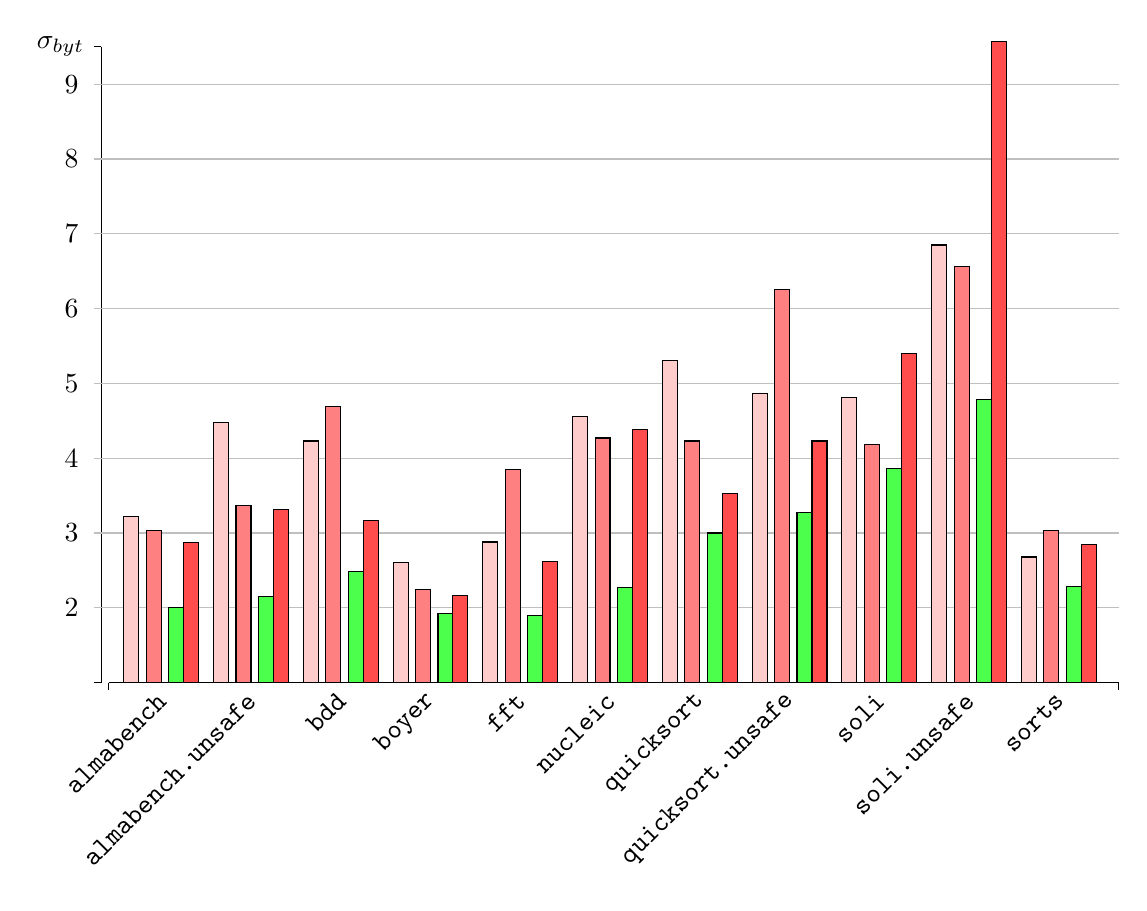
\begin{tikzpicture}[scale=.95]
    \definecolor{color}{HTML}{483D8B}
    \draw (0cm,0cm) -- (13.5cm,0cm);  %Abzisse
    \draw (0cm,0cm) -- (0cm,-0.1cm);  %linkes Ende der Abzisse
    \draw (13.5cm,0cm) -- (13.5cm,-0.1cm);  %rechtes Ende der Abzisse
    \draw (-0.1cm,0cm) -- (-0.1cm,8.5cm);  %Ordinate
    \draw (-0.1cm,0cm) -- (-0.2cm,0cm);  %unteres Ende der Ordinate
    \draw (-0.1cm,8.5cm) -- (-0.2cm,8.5cm) node [left] {$\sigma_{byt}$};  %oberes Ende der Ordinate
    \foreach \x in {2,...,9}
    {
      \draw[gray!50, text=black] (-0.2 cm,\x cm - 1cm) -- (13.5 cm,\x cm - 1cm) node at (-0.5 cm,\x cm - 1cm) {\x};
    }
    \foreach \name/\x/\a/\b/\c/\d in
    {
      almabench/0 / 3.22 / 3.03 / 2.00/2.87,
      almabench.unsafe/1 / 4.48 / 3.37 / 2.15/3.32,
      bdd/2 / 4.23 / 4.69 / 2.48/3.17,
      boyer/3 / 2.61 / 2.24 / 1.93/2.16,
      fft/4 / 2.88 / 3.85 / 1.90/2.62,
      nucleic/5 / 4.56 / 4.27 / 2.27/4.39,
      quicksort/6 / 5.31 / 4.23 / 3.00/3.53,
      quicksort.unsafe/7 / 4.86 / 6.25 / 3.28/4.23,
      soli/8 / 4.81 / 4.18 /  3.86/5.40,
      soli.unsafe/9 / 6.85 / 6.56 / 4.79/9.57,
      sorts/10 / 2.68 / 3.03 / 2.29/2.85
    }
    {
      \pgfmathsetmacro\xinc{0.2}
      \pgfmathsetmacro\xoff{\x * 1.2 + \xinc}
      \pgfmathsetmacro\aoff{\a - 1.0}
      \pgfmathsetmacro\boff{\b - 1.0}
      \pgfmathsetmacro\coff{\c - 1.0}
      \pgfmathsetmacro\doff{\d - 1.0}
      \draw[fill=red!20] (\xoff cm + 0 * \xinc cm, 0 cm) rectangle (1 * \xinc cm + \xoff cm, \aoff);
      \draw[fill=red!50] (\xoff cm + 1 * \xinc cm + .1cm, 0 cm) rectangle (2 * \xinc cm + \xoff cm + .1cm, \boff);
      \draw[fill=green!70] (\xoff cm + 2 * \xinc cm + .2cm, 0 cm) rectangle (3 * \xinc cm + \xoff cm + .2cm, \coff);
      \draw[fill=red!70] (\xoff cm + 3 * \xinc cm + .2cm, 0 cm) rectangle (4 * \xinc cm + \xoff cm + .2cm, \doff);
      \node[rotate=45,left] at (\xoff cm + 3 * \xinc cm, -.1cm) {\texttt{\name}};
    };
  \end{tikzpicture}
  \caption{Speedup relative to the byte-code interpreter}
  \label{figure:Speedup_relative_to_the_byte_code_interpreter}
\end{figure*}

\begin{figure*}[h]
  \centering
  \footnotesize
  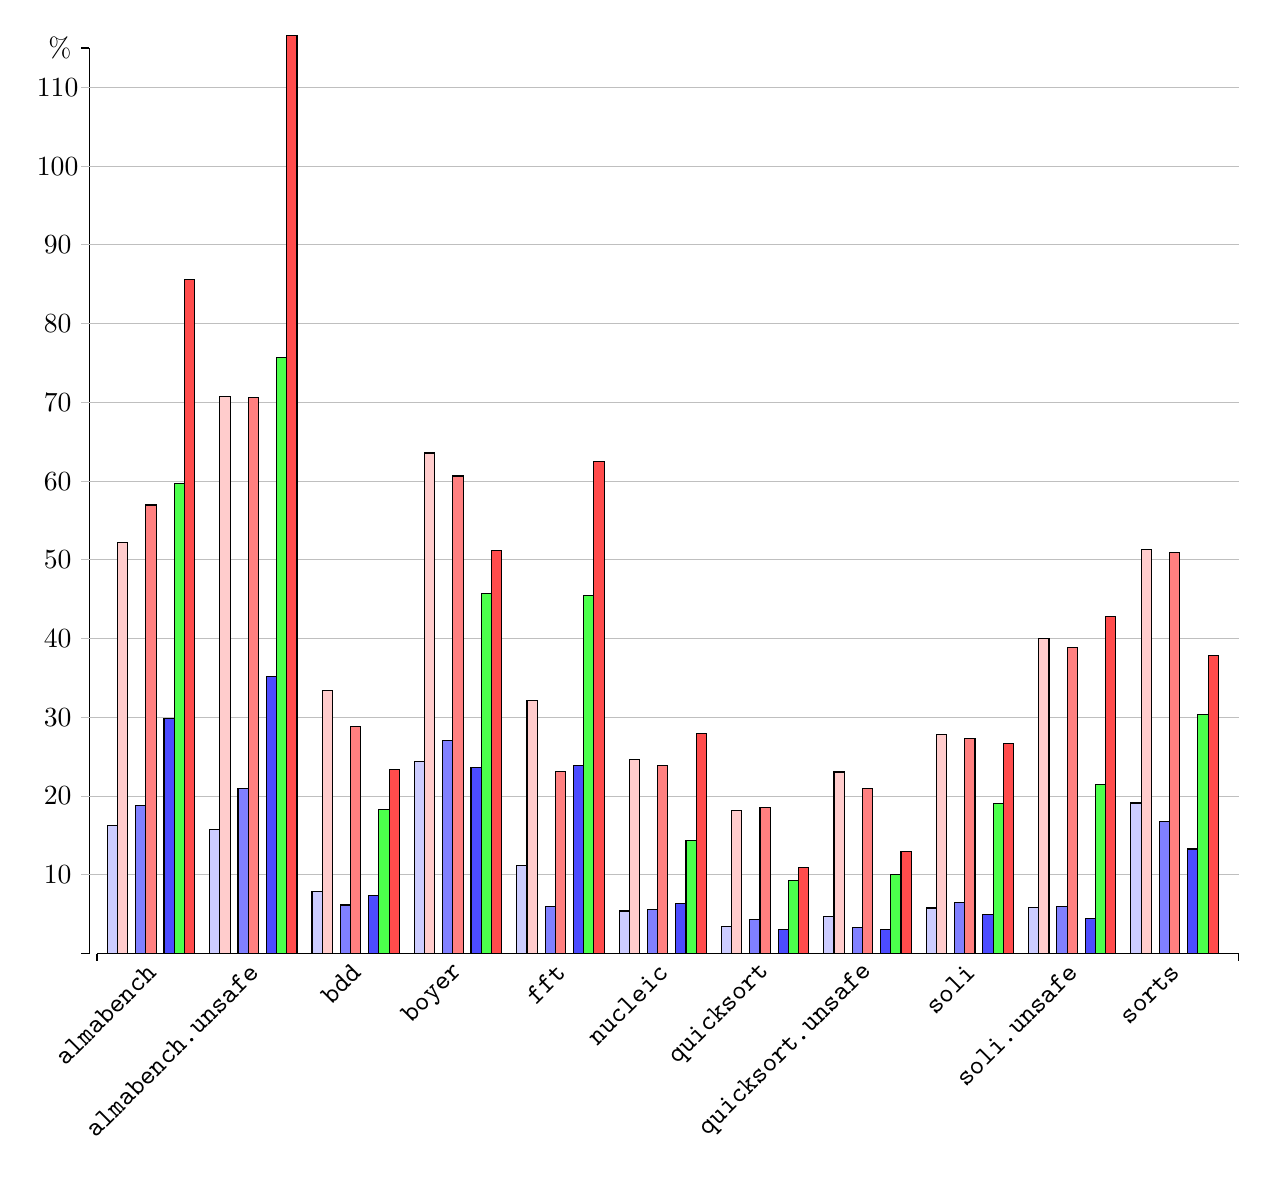
\begin{tikzpicture}
    \definecolor{color}{HTML}{483D8B}
    \draw (0cm,0cm) -- (14.5cm,0cm);  %Abzisse
    \draw (0cm,0cm) -- (0cm,-0.1cm);  %linkes Ende der Abzisse
    \draw (14.5cm,0cm) -- (14.5cm,-0.1cm);  %rechtes Ende der Abzisse
    \draw (-0.1cm,0cm) -- (-0.1cm,11.5cm);  %Ordinate
    \draw (-0.1cm,0cm) -- (-0.2cm,0cm);  %unteres Ende der Ordinate
    \draw (-0.1cm,11.5cm) -- (-0.2cm,11.5cm) node [left] {\%};  %oberes Ende der Ordinate
    \foreach \y in {1,...,11}  %Hilfslinien
    {
      \pgfmathtruncatemacro\ytext{\y * 10}
      \draw[gray!50, text=black] (-0.2 cm,\y cm) -- (14.5 cm,\y cm)
        node at (-0.5 cm,\y cm) {\ytext};  %Beschriftung
    };
    \foreach \name/\x/\a/\b/\c/\d/\e/\f/\g in
    {
      almabench/0 / 1.621/5.218 / 1.878/5.696 / 2.981/5.971/8.564,
      almabench.unsafe/1 / 1.579/7.079 / 2.097/7.065 / 3.513/7.567/11.662,
      bdd/2 / 0.790/3.340 / 0.616/2.888 / 0.738/1.830/2.337,
      boyer/3 / 2.435/6.357 / 2.703/6.065 / 2.363/4.572/5.115,
      fft/4 / 1.116/3.212 / 0.602/2.316 / 2.389/4.544/6.254,
      nucleic/5 / 0.540/2.461 / 0.560/2.390 / 0.636/1.441/2.794,
      quicksort/6 / 0.342/1.817 / 0.438/1.854 / 0.311/0.933/1.098,
      quicksort.unsafe/7 / 0.475/2.306 / 0.336/2.098 / 0.306/1.004/1.294,
      soli/8 / 0.578/2.778 / 0.652/2.727 / 0.494/1.905/2.667,
      soli.unsafe/9 / 0.584/4.000 / 0.593/3.889 / 0.448/2.143/4.286,
      sorts/10 / 1.912/5.131 / 1.679/5.095 / 1.328/3.038/3.785
    }
    {
      \pgfmathsetmacro\xinc{0.13}
      \pgfmathsetmacro\xoff{\x * 1.3 + \xinc}
      \draw[fill=blue!20] (\xoff cm + 0 * \xinc cm, 0 cm) rectangle (1 * \xinc cm + \xoff cm, \a);
      \draw[fill=red!20] (\xoff cm + 1 * \xinc cm, 0 cm) rectangle (2 * \xinc cm + \xoff cm, \b);
      \draw[fill=blue!50] (\xoff cm + 2 * \xinc cm + .1cm, 0 cm) rectangle (3 * \xinc cm + \xoff cm + .1cm, \c);
      \draw[fill=red!50] (\xoff cm + 3 * \xinc cm + .1cm, 0 cm) rectangle (4 * \xinc cm + \xoff cm + .1cm, \d);
      \draw[fill=blue!70] (\xoff cm + 4 * \xinc cm + .2cm, 0 cm) rectangle (5 * \xinc cm + \xoff cm + .2cm, \e);
      \draw[fill=green!70] (\xoff cm + 5 * \xinc cm + .2cm, 0 cm) rectangle (6 * \xinc cm + \xoff cm + .2cm, \f);
      \draw[fill=red!70] (\xoff cm + 6 * \xinc cm + .2cm, 0 cm) rectangle (7 * \xinc cm + \xoff cm + .2cm, \g);
      \node[rotate=45,left] at (\xoff cm + 5 * \xinc cm, -.1cm) {\texttt{\name}};
    };
  \end{tikzpicture}
  \caption{Performance relative to \texttt{ocamlopt}}
  \label{figure:Performance_relative_to_ocamlopt}
\end{figure*}



%% Future work
\section{Future work} \label{section:Future_work}

TODO


%% Conclusion
\section{Conclusion} \label{section:Conclusion}

TODO


%% Acknowlegdements
\section*{Acknowledgements}

TODO


%% References
\bibliographystyle{habbrv}
\bibliography{citations}

\end{document}
